\section{Methods}
\label{sec:methods}

Here, we developed an agentic resource allocation framework to investigate dynamic exploration-exploitation balancing in batch multi-objective Bayesian optimization (MOBO) under evolving constraints. The framework comprises three integrated components: (i) high-fidelity ground truth models providing computationally tractable experiment proxies, (ii) a batch MOBO engine for candidate selection, and (iii) a resource allocation layer governing the exploration–exploitation balance at each iteration. We evaluate this framework on two multi-objective alloy composition optimization problems that serve as realistic test cases with competing objectives, discrete design spaces, and resource constraints representative of experimental materials discovery campaigns. Figure~\ref{fig:workflow} illustrates the overview of the agentic resource allocation framework and the interaction of these components within a complete optimization campaign.

\begin{figure}
    \centering
    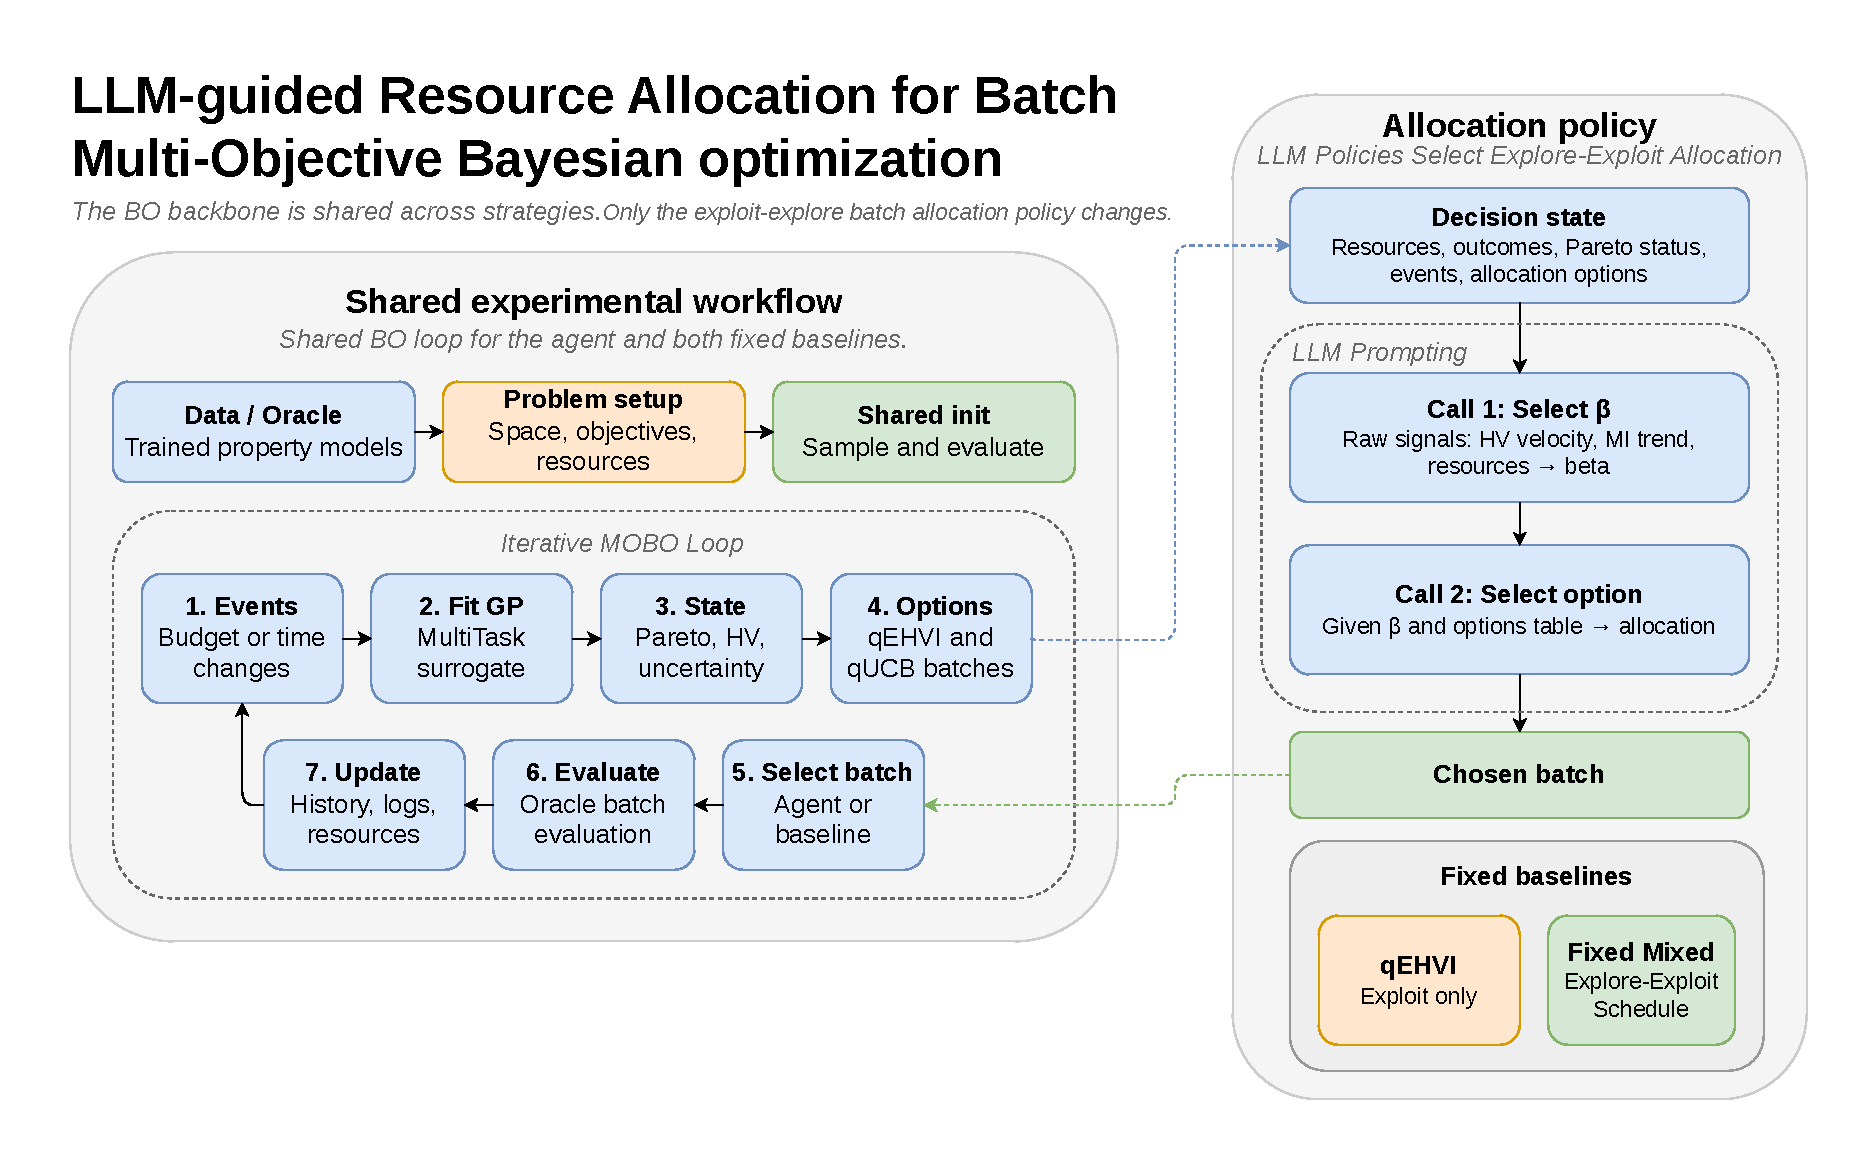
\includegraphics[width=1\linewidth]{figures/workflow.pdf}
    \caption{Overview of the developed LLM-guided resource allocation framework for batch multi-objective Bayesian optimization. The optimization loop is shared across all methods: surrogate fitting, state estimation, allocation-option generation, batch evaluation, and update. The proposed agent selects among exploit-explore batch allocations based on the current decision state, whereas the baselines use fixed qEHVI-only or qUCB-only allocations.}
    \label{fig:workflow}
\end{figure}

% -----------------------------------------------------------------------

\subsection{Test Problems: Alloy Composition Optimization}
\label{sec:problems}

The two systems evaluated comprised a three-objective problem in a high-dimensional multi-component soft-magnetic alloy composition space and a two-objective problem over a septenary refractory high-entropy alloy (RHEA) space.

The Fe-Co-Ni-based multi-component soft-magnetic alloy system was optimized by maximizing saturation magnetization $M_s$ in T, minimizing the logarithm of coercivity $\log_{10} H_c$ in A/m, and maximizing the logarithm of Vickers hardness $\log_{10} H_V$. High $M_s$ drives magnetic flux density, low $H_c$ reduces hysteresis losses, and sufficient $H_V$ ensures mechanical integrity, which together define the core trade-off surface for soft-magnetic applications such as transformers, inductors, and electromagnetic actuators~\cite{padhy2024experimentally}. The composition space comprises three primary elements (Fe, Co, Ni), each ranging over [0, 100] at.\%, subject to a group constraint requiring their sum to fall within [90, 100] at.\%, and six dopant elements (V, Mo, C, Nb, Ti, Si), each at most 5 at.\%, with their combined contribution constrained to at most 10 at.\%. All elements are sampled at 2 at.\% increments under these group constraints, yielding exactly 331,227 unique valid compositions. Training data were sourced from~\cite{padhy2024experimentally}. This literature-compiled database contains many compositions reported multiple times under different processing conditions, which composition-only inputs cannot distinguish, and its missing property values were imputed by Padhy \etal\ using property-specific machine learning models.

\label{sec:mpd-problem}
The septenary Ti-V-Nb-Mo-Hf-Ta-W refractory HEA (RHEA) system was optimized by maximizing melting temperature $T_m$ in K and minimizing density $\rho$ in g\,cm$^{-3}$ ~\cite{hastings2025leveraging}. High-temperature, low-density refractory alloys are of high interest for high-temperature structural applications such as aerospace propulsion applications~\cite{SENKOV20101758, ZHUO20241097}. Per-element bounds are Ti [0,35], V [0,50], Nb [22.5,67.5], Mo [0,12.5], Hf [0,12.5], Ta [0,45], W [0,12.5] at.\%, sampled at 5 at.\% spacing under the simplex constraint, yielding exactly 9,454 unique compositions.

% -----------------------------------------------------------------------

\subsection{Ground Truth Models}
\label{sec:truth-models}

To enable the large-scale, multi-seed comparative study presented here, spanning hundreds of individual optimization campaigns, ground truth models were developed to serve as computational proxies for experimental evaluation. These ground truth models provide rapid and deterministic predictions for material properties. When the BO loop proposes a composition, the model returns objective values treated as exact experimental measurements.

Model construction was performed using ARMOTE-MO (Automated Regression workflow with Multi-Objective hyperparameter optimization using Tree-Parzen Estimator for Multi-Output regression), a framework that automates the end-to-end multi-output regression workflow, including data preprocessing, hyperparameter optimization, model training, and evaluation. ARMOTE-MO extends our previously developed automated regression workflow (ARW)~\cite{padhy2025automated,saurabh2026automated} to multi-output regression with multi-objective hyperparameter optimization. For both alloy systems, ARMOTE-MO trained a multi-output Random Forest Regressor (RFR)~\cite{Breiman2001} using scikit-learn~\cite{Pedregosa2011}, jointly predicting all objectives. A RFR model was selected owing to its strong baseline performance on tabular compositional data, computational tractability at the dataset scales used here ($10^4$--$10^5$ compositions), and native multi-output support without wrapper overhead. 

The framework manages train/test splitting (80/20) and standardizes inputs to zero mean and unit variance and scales outputs internally, ensuring fair comparison across properties with different physical units and magnitudes. Hyperparameters were optimized via multi-objective Bayesian optimization using Optuna~\cite{Akiba2019} with the Tree-Parzen Estimator (TPE), simultaneously minimizing MSE and maximizing $R^2$ across both outputs through 5-fold cross-validation on scaled split train dataset. This dual-objective search produces a Pareto front of hyperparameter configurations, from which the configuration with the highest mean $R^2$ across both objectives is selected.
The optimal hyperparameters for each system are listed in Table~\ref{tab:rfr-hyperparameters}. The complete ARMOTE-MO algorithm and full hyperparameter search spaces are provided in Appendix~\ref{app:armote}.

\begin{table}[h]
\centering
\begin{tabular}{lcccc}
\toprule
System & $n_\text{trees}$ & max\_depth & min\_samples\_split & min\_samples\_leaf \\
\midrule
RHEA & 53 & 56 & 3 & 1 \\
Fe-Co-Ni        & 134 & 113 & 7 & 1 \\
\bottomrule
\end{tabular}
\caption{Optimal RFR hyperparameters for each alloy system selected by ARMOTE-MO.}
\label{tab:rfr-hyperparameters}
\end{table}

Both models achieve strong predictive accuracy, as confirmed by the parity plots in Fig.~\ref{fig:parity-plots}. Test $R^2$ values for the Fe-Co-Ni magnet system were $M_s$: 0.97, $\log H_c$: 0.91, and $\log H_V$: 0.77. For the RHEA system, $T_m$: 0.89 and $\rho$: 0.93. The lower $\log H_V$ accuracy reflects the greater scatter in hardness measurements across the dopant composition space, though the model captures the broad trends sufficient for comparative strategy evaluation. The slightly lower $T_m$ accuracy reflects the difficulty of predicting melting temperature across a wide compositional range, though the model captures the broad trends sufficient for comparative strategy evaluation. Prior to their use as inputs to the GP surrogate (Section~\ref{sec:gp}), all model outputs are standardized to improve numerical conditioning. Standardization statistics (per-objective mean and standard deviation) are estimated from 100 compositions sampled via quasi-random Sobol sequences from the enumerated design space and held fixed across all strategies and random seeds, ensuring that hypervolume values and GP length scales remain numerically consistent throughout the comparative study.
\begin{figure}[htbp]
    \centering
    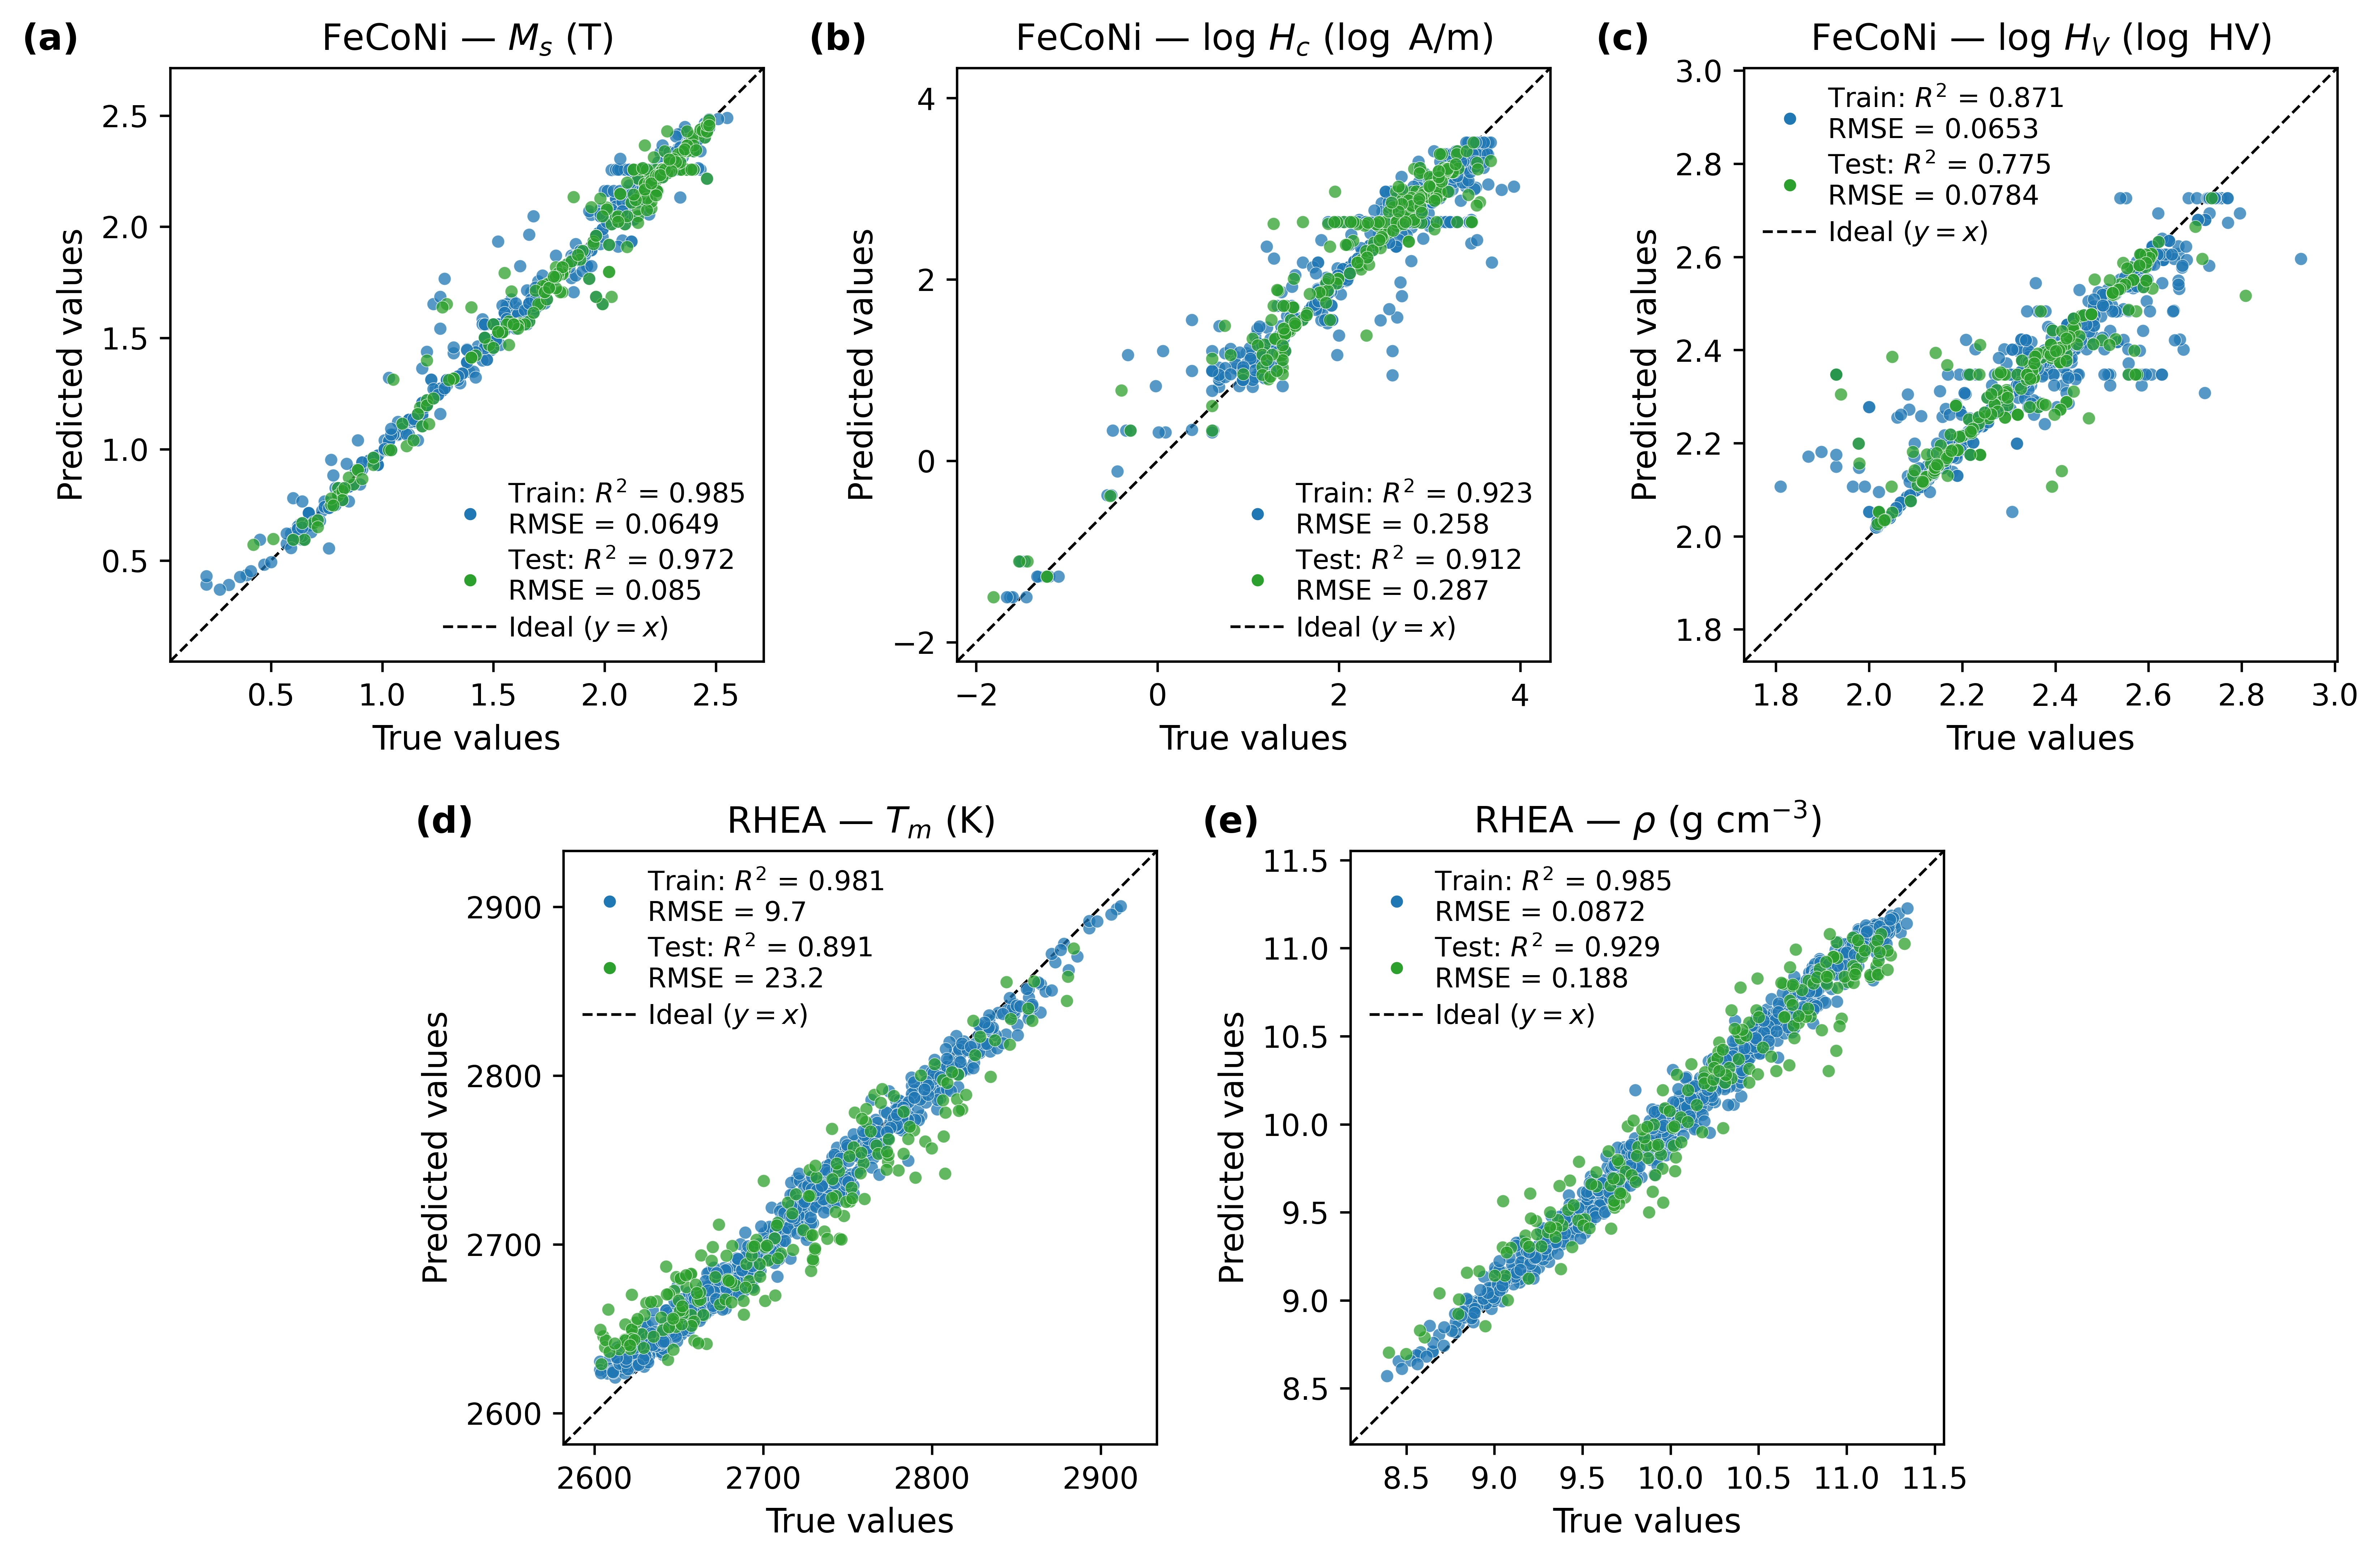
\includegraphics[width=1\linewidth]{figures/fig2_parity_plots.png}
    \caption{Parity plots for the ground truth random forest regression models. Panels (a)--(c) show the Fe--Co--Ni--V--Mo--C--Nb--Ti--Si soft magnetic system with predicted versus measured values for $M_s$ (T, $R^2 = 0.97$), $\log H_c$ ($\log(\text{A/m})$, $R^2 = 0.91$), and $\log H_V$ ($\log(\text{HV})$, $R^2 = 0.77$). Panels (d)--(e) show the Ti--V--Nb--Mo--Hf--Ta--W refractory system with predicted versus measured values for $T_m$ (K, $R^2 = 0.89$) and $\rho$ (g/cm$^3$, $R^2 = 0.93$). The dashed line indicates perfect agreement.}
    \label{fig:parity-plots}
\end{figure}
% -----------------------------------------------------------------------

\subsection{Batch Multi-Objective Bayesian Optimization (MOBO) Engine}
\label{sec:bo-framework}

The batch MOBO engine is embedded within the broader resource allocation framework described in Section~\ref{sec:allocation-framework}. Each iteration begins with fitting a GP surrogate on accumulated data, constructing candidate batches with varying exploration–exploitation mixtures, selecting one batch via the resource allocator, evaluating the selected compositions, and updating the resource state.

All valid compositions are enumerated exhaustively at the specified grid spacings (Section~\ref{sec:problems}). Acquisition functions are optimized exactly over this finite discrete candidate set using BOTorch's~\cite{Balandat2020} \texttt{optimize\_acqf\_discrete}, eliminating continuous relaxation of the simplex constraint and ensuring grid-aligned proposals.

\label{sec:gp}
\texttt{MultiTaskGP}~\cite{Balandat2020,Bonilla2008,Swersky2013} from BOTorch is used to model both objectives jointly at each iteration, capturing inter-objective correlations through shared covariance. Observations from both objectives are interleaved into a single training set by appending a scalar task index to each input composition. Given $n$ evaluated compositions and $d$ elemental components, the training input matrix has shape $(2n,\, d+1)$ and the target vector has shape $(2n,\, 1)$, containing standardized objective values concatenated in task order. The GP hyperparameters are optimized by maximizing the marginal log-likelihood~\cite{Rasmussen2006} at each iteration. Input compositions are normalized to the unit hypercube based on per-dimension design space bounds prior to GP fitting and acquisition function evaluation.

\label{sec:acqf}
We use two acquisition functions to define the exploration–exploitation spectrum and serve as the building blocks for the allocation options:
\begin{itemize}

    \item Exploitation - qExpectedHypervolumeImprovement (qEHVI)~\cite{Daulton2020} measures expected increase in Pareto front hypervolume from a batch of $q$ compositions, estimated via a specified number (256 in our case) of Sobol quasi-Monte Carlo samples~\cite{Joe2008,Balandat2020}. It directs experiments toward known Pareto front improvements and thus operationalizes pure exploitation.

    \item Exploration - qUpperConfidenceBound (qUCB)~\cite{Wilson2017} balances high predicted values and high uncertainty via exploration coefficient $\beta=2.0$, applied to a linearly scalarized combination of both objectives with equal weights of 0.5. To prevent clustering with qEHVI candidates, we add a distance-based diversity bonus:
    \begin{equation}
    \label{eq:ucb-diversity}
    \text{UCB}_{\text{eff}}(\mathbf{x}) = \text{UCB}(\mathbf{x}) + \lambda \min_{\mathbf{x}' \in \mathcal{X}_{\text{qEHVI}}} \|\mathbf{x} - \mathbf{x}'\|_2
    \end{equation}
    where $\mathcal{X}_{\text{qEHVI}}$ are the set of candidates already selected by qEHVI in the current allocation option and $\lambda=1.0$ is the diversity weight. This drives qUCB toward regions of the design space that are geometrically distant from qEHVI candidates, ensuring that exploration and exploitation compositions cover complementary areas of composition space within each batch.

\end{itemize}

\label{sec:reference-point}
A fixed reference point $\mathbf{r}$ for hypervolume calculation is computed once by evaluating the full enumerated design space through the ground truth model and taking the per-objective minimum minus a margin of 0.1 in the post-processed objective space. This fixed $\mathbf{r}$ is shared across all strategies and seeds, ensuring that hypervolume values are directly comparable throughout the study.

% -----------------------------------------------------------------------

\subsection{Resource Allocation Layer}
\label{sec:allocation-framework}

As mentioned in the Introduction, the core contribution is a resource allocation layer that determines how to split experimental effort between exploration and exploitation per batch at each iteration. Rather than fixing this split, the framework enumerates all feasible mixtures, characterizes each with exploration and exploitation metrics, and delegates selection to a resource allocator (fixed policy or LLM agent). This separates which compositions to evaluate from how to balance strategies over time, enabling dynamic policy control without modifying the MOBO engine.

Given a batch size $q$, we define $q+1$ allocation options indexed $i = 0, 1, \ldots, q$. Option $i$ allocates $q - i$ compositions to qEHVI (exploitation) and $i$ compositions to qUCB (exploration). Options are constructed sequentially. For option $i$, qEHVI first selects $q-i$ exploitation compositions; these are passed to qUCB as the anchor set $\mathcal{X}_\mathrm{qEHVI}$ in Eq.~\eqref{eq:ucb-diversity}, which then selects $i$ exploration compositions with diversity awareness. Therefore, option 0 is pure exploitation; option $q$ is pure exploration; intermediate options represent partial mixtures spanning the full exploration--exploitation spectrum. % 
For both the RHEA and Fe-Co-Ni magnet experiments, we use $q = 5$, yielding six options (5+0, 4+1, 3+2, 2+3, 1+4, 0+5).

Each allocation option is characterized by two scalar metrics that together describe the expected utility from exploitation and exploration perspectives. These metrics are computed from the current GP surrogate before any evaluation occurs and are provided to the resource allocator as the basis for its decision.

\begin{itemize}

    \item Expected Hypervolume Improvement (EHVI) - The EHVI of an allocation quantifies the expected increase in the dominated hypervolume of the Pareto front if the combined batch were evaluated:
    \begin{equation}
    \label{eq:ehvi}
    \mathrm{EHVI}(X_S) = \mathbb{E}\!\left[
        \mathrm{HV}\!\left(\mathcal{Y}_\mathrm{obs} \cup f(X_S),\, \mathbf{r}\right)
        - \mathrm{HV}\!\left(\mathcal{Y}_\mathrm{obs},\, \mathbf{r}\right)
    \right]
    \end{equation}
    where $X_S$ is the $q$-composition batch, $f(\cdot)$ is the unknown objective function, $\mathcal{Y}_\mathrm{obs}$ is the set of all previously observed objective values, $\mathrm{HV}(\cdot, \mathbf{r})$ denotes the hypervolume dominated relative to reference point $\mathbf{r}$, and the expectation is taken over the GP posterior. EHVI is estimated by evaluating the qEHVI acquisition function on the combined batch $X_S$ using the current surrogate, regardless of which compositions in $X_S$ originated from qEHVI vs. qUCB. A high EHVI value indicates that the batch is well-positioned to substantially advance the known Pareto front.

    \item Mutual Information (MI) - The MI quantifies the expected reduction in uncertainty about the Pareto-optimal region of the objective space resulting from evaluating the batch $X_S$. Formally, it is the mutual information between the GP predictive distribution at $X_S$ and a sample from the surrogate Pareto-optimal set:

    \begin{equation}
    \label{eq:mi}
    \mathrm{MI}(X_S) = H\!\left(f(X_S)\right)
        - \frac{1}{\tilde{M}} \sum_{m=1}^{\tilde{M}} H\!\left(f(X_S) \mid f(\mathbf{x}^*_m)\right)
    \end{equation}
    where $\mathbf{x}^*_m$, $m = 1, \ldots, \tilde{M}$, are Monte Carlo samples from the surrogate Pareto-optimal set (we use $\tilde{M}$ here to distinguish the number of Pareto samples from the number of objectives $M$) and $H(\cdot)$ denotes differential entropy~\citep{Cover2006}. Under the Gaussian posterior of the MultiTaskGP, both entropy terms are computed analytically. For the joint distribution over $X_S$ evaluated at all $M$ objectives, the GP covariance matrix has dimension $Mq \times Mq$ ($M$ tasks, $q$ compositions per task). The prior entropy is:
    \begin{equation}
    \label{eq:prior-entropy}
    H\!\left(f(X_S)\right)
        = \frac{1}{2}\!\left[ Mq\ln(2\pi e) + \ln \left|\boldsymbol{\Sigma}_\mathrm{prior}\right| \right]
    \end{equation}
    where $\boldsymbol{\Sigma}_\mathrm{prior}$ is the $Mq \times Mq$ GP posterior covariance at the task-augmented inputs for $X_S$. After conditioning on a hypothetical observation at $\mathbf{x}^*_m$, the conditional entropy is:
    \begin{equation}
    \label{eq:cond-entropy}
    H\!\left(f(X_S) \mid f(\mathbf{x}^*_m)\right)
        = \frac{1}{2}\!\left[ Mq\ln(2\pi e)
            + \ln \left|\boldsymbol{\Sigma}_\mathrm{prior}
                - \boldsymbol{\Sigma}_{12}\boldsymbol{\Sigma}_{22}^{-1}\boldsymbol{\Sigma}_{21}
            \right| \right]
    \end{equation}
    where $\boldsymbol{\Sigma}_{12}$ is the $Mq \times M$ cross-covariance between $X_S$ and $\mathbf{x}^*_m$, $\boldsymbol{\Sigma}_{22}$ is the $M \times M$ posterior covariance at $\mathbf{x}^*_m$, and the Schur complement $\boldsymbol{\Sigma}_\mathrm{prior} - \boldsymbol{\Sigma}_{12}\boldsymbol{\Sigma}_{22}^{-1}\boldsymbol{\Sigma}_{21}$ is the conditional covariance of $f(X_S)$ given an observation at $\mathbf{x}^*_m$. A regularization term of $10^{-6}\mathbf{I}$ is added to all covariance matrices before computing log-determinants for numerical stability. The $\tilde{M} = 10$ surrogate Pareto samples are obtained by: (1) drawing 1000 compositions using Sobol sampling from the design space, (2) drawing a joint GP posterior sample path over the 1000 compositions for all $M$ objectives, (3) identifying the non-dominated set of these sampled objective vectors, and (4) drawing one composition uniformly from that set. This procedure is repeated $\tilde{M}$ times independently.

    MI is computed for each allocation option independently before any evaluation occurs, and we track both per-iteration and cumulative MI across the campaign as a measure of landscape characterization breadth. In real discovery campaigns, future constraints, objectives, or target regions are rarely fully known at the outset. A strategy that generates higher MI leaves behind a more thoroughly characterized landscape, broadening the range of Pareto-adjacent compositions that can be identified if campaign priorities shift. The default $\beta = 2$ used for qUCB tends to select compositions near the current Pareto boundary, where predicted values are high and uncertainty is moderate. When $\beta$ is elevated, proposals shift toward more speculative, high-uncertainty regions that are not necessarily close to the current front. MI remains a meaningful characterization measure in both regimes, as it quantifies the reduction in GP uncertainty about the Pareto-optimal region regardless of how close the proposed compositions are to the current front.

\end{itemize}

Within the resource allocation decision, EHVI values are compared across options to rank exploitation potential, and MI values are compared across options to rank exploration value. The resource allocator receives both metrics as inputs and is explicitly instructed to treat them as separate ordinal signals.

% -----------------------------------------------------------------------
\subsection{Resource Allocation Strategies}
\label{sec:strategies}

We compared four resource allocation strategies that differ in how they select among the $q+1$ allocation options at each iteration. First are two fixed-policy baselines that require no campaign history.

The first strategy, called \textit{qEHVI} for simplicity, always selects option $i = 0$, directing the entire batch to the qEHVI acquisition function. This strategy serves as a reference for purely greedy acquisition behavior.

Next, the \textit{Fixed Mixed} strategy stages the allocation according to a deterministic schedule based on the fraction of resources remaining. When more than 75\% of total budget and time remain, it selects pure exploration (option $q$). For 25 to 75\% remaining, it selects the middle option, corresponding to 3 exploitation points and 2 exploration points for $q=5$. Below 25\%, it switches to pure exploitation (option 0). The exploration coefficient is fixed at $\beta = 2.0$ throughout. This policy captures a commonly applied experimental heuristic of exploring broadly early and then committing to the best-known region without requiring any learning or feedback.

The remaining two strategies are LLM-based agents designed to adapt to accumulated campaign evidence each iteration.

The \textit{Rule-Swap} strategy is an LLM-based agent whose primary objective is to maximize hypervolume as efficiently as possible, treating exploration as a targeted response to specific optimization failure modes rather than a routine investment at every iteration. The agent's primary diagnostic signal is hypervolume gain per newly added Pareto point (HV/pt) observed in recent qEHVI-dominant iterations. The agent defaults to pure qEHVI allocation and deviates only when the HV/pt trend shows crowding, where returns on new Pareto points are diminishing and qEHVI is refining known territory rather than expanding, or stagnation, where no new Pareto points have been added across several consecutive iterations. The degree of exploration added scales with the severity of the signal. The decision framing for when and how much to explore is encoded in the prompt rather than in Python control flow, so the LLM makes the actual judgment call within that framing. The agent makes two sequential LLM calls per iteration, with Call 1 producing a stagnation assessment and selecting $\beta$, and Call 2 selecting the allocation option using the resulting options table. Full prompt details are provided in Appendix~\ref{app:prompts}.

\textit{Adaptive-$\beta$} takes a broader view of campaign state. Rather than a single diagnostic, it evaluates the HV velocity ratio (recent mean $\Delta$HV relative to the historical baseline), the current MI value relative to its value at the start of the campaign, per-element composition ranges across the current Pareto front to support domain reasoning about which regions of composition space have been covered, and a rolling six-iteration history of decisions and outcomes. Call 1 selects $\beta$ based on these signals. Call 2 then selects among the $q+1$ allocation options constructed at that $\beta$, guided by the Call 1 reasoning and the options table of qEHVI and MI scores. Unlike Rule-Swap, no fixed decision rules are encoded in the prompt. The LLM receives principled guidance text alongside raw computed signals and makes unconstrained decisions, with Python enforcement limited to output parsing and bounding the option index to $[0,q]$. All LLM calls for both agents use GPT-4o~\citep{OpenAI2024} (OpenAI API model identifier \texttt{gpt-4o}, queried 24--29 June 2026) through the LangChain~\citep{Chase2022} API. Full prompt details are provided in Appendix~\ref{app:prompts}.

Resource events are mid-campaign modifications to budget or time constraints applied at a specified iteration, designed to simulate realistic laboratory disruptions such as unexpected funding reductions or shortened project timelines. The two fixed-policy baselines, qEHVI and Fixed Mixed, have no mechanism to respond and continue executing their schedules regardless of constraint changes. Both LLM-based agents receive notification of an event in the second LLM call at the iteration the event occurs, as well as a one-iteration advance warning in the preceding prompt (Appendix~\ref{app:prompts_events}), giving them the opportunity to adjust allocation before the constraint takes effect.
 
% -----------------------------------------------------------------------
\subsection{Experimental Design}
\label{sec:experimental-design}

Each optimization campaign begins with $n_\mathrm{init}$ compositions sampled uniformly at random from the enumerated discrete design space, evaluated through the ground truth model to produce the initial training dataset for the GP surrogate. The same $n_\mathrm{init}$ compositions and their corresponding objective values are shared across all four strategies within a given random seed, ensuring that differences in strategy performance reflect allocation decisions made during the campaign rather than differences in starting conditions. A new random initialization is drawn independently for each seed, with $n_\mathrm{init} = 15$ for the Fe-Co-Ni magnet experiments to accommodate the larger compositional search space and three-objective structure, and $n_\mathrm{init} = 5$ for the RHEA experiments.

All experiment configurations are summarized in Table~\ref{tab:experiments}. Each experiment is run with all four strategies using the same shared initialization per seed.

The two baseline experiments establish primary baselines comparing strategies in an unconstrained setting, while the six event experiments test strategy adaptability under mid-campaign resource variations where one or two constraint reductions are introduced during the early-to-mid phase of each campaign. These events are timed to fall when per-iteration gains are still substantial, creating the strongest test of whether the agent can recognize and respond to sudden changes in constraints. The baseline campaigns were designed such that the time and budget constraints will equally constrain the campaign. 

\begin{table}[h]
\centering
\begin{tabular}{llccccp{4.5cm}}
\toprule
Experiment         & System                     & Seeds & Iters & $q$ & $n_\mathrm{init}$ & Event(s) \\
\midrule
MP-D-MAIN     & RHEA & 25   & 55    & 5   & 5 & None \\
MP-D-BUDGET   & RHEA & 25   & 55    & 5   & 5 & Budget cut at iter.\ 15 \\
MP-D-TIME     & RHEA & 25   & 55    & 5   & 5 & Time cut at iter.\ 15 \\
MP-D-DUAL     & RHEA & 25   & 55    & 5   & 5 & Time cut at iter.\ 5; budget cut at iter.\ 7 \\
Magnets-MAIN   & Fe-Co-Ni & 25  & 50    & 5   & 15 & None \\
Magnets-BUDGET & Fe-Co-Ni & 25  & 50    & 5   & 15 & Budget cut at iter.\ 18 \\
Magnets-TIME   & Fe-Co-Ni & 25  & 50    & 5   & 15 & Time cut at iter.\ 13 \\
Magnets-DUAL   & Fe-Co-Ni & 25  & 50    & 5   & 15 & Time cut at iter.\ 13; budget cut at iter.\ 18 \\
\bottomrule
\end{tabular}
\caption{Summary of all experiment configurations. \textit{Iters} denotes the maximum number of BO iterations; campaigns with resource events terminate earlier when a constraint is exhausted. $q$ denotes batch size. $n_\mathrm{init}$ denotes the number of initial compositions shared across all strategies within each seed.
}
\label{tab:experiments}
\end{table}

The primary evaluation metric is the hypervolume indicator of the Pareto front approximation~\citep{Zitzler1998}. Given the fixed reference point $\mathbf{r} \in \mathbb{R}^M$ and the set of non-dominated evaluated compositions $\mathcal{Y}_\mathrm{pareto}$ accumulated through iteration $t$, the hypervolume is:
%
\begin{equation}
\label{eq:hypervolume}
\mathrm{HV}(\mathcal{Y}_\mathrm{pareto}, \mathbf{r})
    = \lambda\!\left(
        \left\{
            \mathbf{y} \in \mathbb{R}^M \;\middle|\;
            \mathbf{r} \preceq \mathbf{y}
            \text{ and }
            \exists\, \mathbf{p} \in \mathcal{Y}_\mathrm{pareto} : \mathbf{y} \preceq \mathbf{p}
        \right\}
    \right)
\end{equation}
%
where $\lambda$ denotes the Lebesgue measure ($M$-dimensional volume) and $\preceq$ denotes component-wise inequality. Larger hypervolume indicates the discovery of both high-performing and diverse alloys in the objective space. For the RHEA problem with $M=2$, the hypervolume is computed over melting point and negated density whereas in the Fe-Co-Ni magnet problem with $M=3$, it is computed over the three-dimensional objective space of $M_s$, $-\log H_c$, and $\log H_V$. In both cases, the fixed reference point described in Section~\ref{sec:reference-point} is used, enabling direct comparison across seeds and strategies within each system. 

To facilitate comparison across two systems with different hypervolume scales, we report hypervolume normalized by the theoretical maximum, specifically the hypervolume of the full design space Pareto front computed by evaluating the ground truth model over all enumerated compositions. This normalized HV lies in $[0, 1]$, where 1.0 corresponds to the best achievable Pareto front given the design space. Mean normalized HV and standard error of the mean across 25 random seeds are reported at each iteration for every strategy-configuration pair. As secondary metrics, the area under the HV curve (AUC-HV) is reported as a summary of early-campaign convergence speed, and cumulative mutual information in nats is reported as a measure of design space characterization breadth.
